%% Abschnitt1.tex
%% $Id: Abschnitt1.tex 28 2007-01-18 16:31:32Z bless $
%%


%% ==============================
\section{Signal}
%% ==============================
Ein Signal bildet eine Vibration ab. Dabei besitzt ein Signal Attribute, die die obengenannte Reaktion darstellen sollten. Als man sich die Einstellungsm{\"o}glichkeiten einer Vibration des Wearable genauer angeguckt hat, hat man festgestellt, dass man die L{\"a}nge und die St{\"a}rke einer Vibration einstellen kann. Das hat zur Folge, dass diese zwei Faktoren als die Attribute eines Signales benutzt wurden um eine Vibration zu repr{\"a}sentieren.

Man stellt sich jetzt die Frage,
Wie lang sollen die Vibrationen denn jetzt sein ? 

Um diese Frage zu beantworten, guckt man sich anhand an dem Paper \cite{pescara2016ruttelflug} die benutzten Vibrationsl{\"a}ngen an. Da wurden die Grenzen zwischen 100 und 1000ms f{\"u}r eine Vibration benutzt. Diese Werte hat man so {\"u}bernommen. Das bedeutet, ein Signal hat eine minimale L{\"a}nge von 100ms und eine maximale L{\"a}nge von 1000 ms. 

Anhand der Hypothese der Bachelorarbeit wolle man wissen, wie gut sich personalisierte Vibrationen im Vergleich zu generischen Vibrationen verbessern. Diese Frage l{\"a}sst sich wie folgt beantworten. Erstens musste man sich {\"u}berlegen, wie man personalisierte Vibrationen mittels dem EA f{\"u}r einen Probanden bestimmen will.
Au{\ss}erdem sollte man herausfinden was f{\"u}r Signale noch gut voneinander unterscheidbar sind, die die Grenzen von 100ms bis 1000ms besitzen.
Man habe sich auf drei Typen von Signalen festgelegt, die als Kurz, Mittel und Lang definiert. Dadurch wolle man wissen, ob ein Signal als Kurz, Mittel oder Lang empfunden wurde.

Die jeweiligen Typen definieren innerhalb der Grenzen von 100ms und 1000ms ein Intervall, das sich voneinander nicht {\"u}berschneiden kann. Abgesehen davon ist der niedrigste Messwert von Lang Signal allgemein gr{\"o}{\ss}er als der h{\"o}chste Messwert von Mittel Signal. Wiederum ist die kleinste Intensit{\"a}t von Mittel Signal ist in der Regel gr{\"o}{\ss}er als die gr{\"o}{\ss}te Internsit{\"a}t von Kurz Signal. Als Beispiel habe man f{\"u}r Kurz die Intervallgrenzen 100ms und 300ms, f{\"u}r Mittel habe man dann die Intervallgrenzen von 400ms bis 600ms und f{\"u}r Lang habe man die Intervallgrenzen von 700ms bis 1000ms. 
Allerdings wurde es darauf geachtet, dass die Grenzen nicht aufeinander liegen, sondern einen Abstand zwischen den Grenzen existiert. Bei der St{\"a}rke einer Vibration wurde man an der Darstellbarkeit des Wearable gebunden. Nachdem man herausgefunden hat, dass man nur die Bereiche von 0x7FFF bis 0xFFFF als merkbare Vibrationsst{\"a}rken besitzt, hat man sich diese Bereiche in 5 Stufen eingeteilt. Daraus folgt dass man sich f{\"u}r den sp{\"a}teren Verlauf f{\"u}nf Zust{\"a}nde definiert. Ein 

\begin{tabular}{lcr}
  Signalst{\"a}rke & Namen & Zustandsnamen \\
  $\mathtt{0x7FFF}$ & Very Weak & $q_{VWeak}$ \\
  $\mathtt{0x9FFF}$ & Weak & $q_{Weak}$ \\
  $\mathtt{0xBFFF}$ & OK & $q_{OK}$ \\
  $\mathtt{0xDFFF}$ & Strong & $q_{Strong}$ \\
  $\mathtt{0xFFFF}$ & Very Strong & $q_{VStrong}$ \\
\end{tabular}


%% ==============================
\section{Muster}
%% ==============================
Ein Muster ist dabei eine Folge von mehreren Signalen.

%% ==============================
\section{Eingabe f{\"u}r den Algorithmus}
%% ==============================
Als Eingabe f{\"u}r den Algorithmus ben{\"o}tigt man eine Population von Individuen. Die Individuen sind in diesem Fall Signale. 
Nicht jede Person empfindet ein vorgegebenes Kurzes Signal gleich wie eine andere Person, somit musste man zuvor den Benutzer befragen, was er als Kurz, Mittel und Lang empfindet. Zuerst habe man alle Signale abgespielt, damit der Proband wusste, was Ihn erwartet. 
Nachdem alle Signale abgespielt wurden, wurde jedes Signal einzeln abgespielt und der Proband hatte die Aufgabe das abgespielte Signal der Kategorie Kurz, Mittel oder Lang zuzuordnen. 
Jedem Probanden wurde insgesamt 10 Signale mit der gleichen Vibrationsst{\"a}rke abgespielt, die Signalel{\"a}nge ist dabei gleich verteilt.
Dabei wurden alle 10 Signale in einer zuf{\"a}lligen Reihenfolge abgespielt.

Nach der Eingabe des Probanden erh{\"a}lt man beispielsweise folgende Bewertung. Diese Eingabe ist ideal, da alle Signaltypen direkt hintereinander vorliegen, so w{\"u}rde man hier ein die Grenzen sofort aus der Tabelle entnehmen k{\"o}nnen. Diese belaufen sich f{\"u}r Kurz zwischen 100 und 300 ms, f{\"u}r Mittel zwischen 400ms und 600ms und f{\"u}r Lang zwischen 700 und 1000ms.

\begin{table}[]
\centering
\caption{My caption}
\label{my-label}
\begin{tabular}{|l|l|l|l|l|l|l|l|l|l|l|}
\hline
 Signall{\"a}nge & 100ms & 200ms & 300ms & 400ms & 500ms & 600ms & 700ms & 800ms & 900ms & 1000ms \\ \hline
 Erkannten Signaltyp & Kurz & Kurz & Kurz & Mittel & Mittel & Mittel & Lang & Lang & Lang & Lang \\ \hline
\end{tabular}
\end{table}

Falls die Eingabe jedoch nicht so Ideal sein sollte, wie in dem Beispiel gerade eben, mussten ein paar Vorkehrungen getroffen werden. Um einige Sonderf{\"a}lle auszuschlie{\ss}en, hat man {\"u}berpr{\"u}ft, ob das Signal mit der L{\"a}nge von 100ms ein Kurzes Signal ist und das Signal mit der L{\"a}nge von 1000ms ein Langes Signal ist, sowie man annimmt, dass mindestens jeder Signaltyp mindesten zwei mal ausgew{\"a}hlt wurde. Sollte dies nicht der Fall sein, so w{\"u}rde man den Benutzer dazu bitten, die zehn Signale erneut zu bewerten. 

\begin{table}[]
\centering
\caption{My caption}
\label{my-label}
\begin{tabular}{|l|l|l|l|l|l|l|l|l|l|l|}
\hline
 Signall{\"a}nge & 100ms & 200ms & 300ms & 400ms & 500ms & 600ms & 700ms & 800ms & 900ms & 1000ms \\ \hline
 Erkannten Signaltyp & Kurz & Kurz & Mittel & Mittel & Lang & Mittel & Lang & Lang & Lang & Lang \\ \hline
\end{tabular}
\end{table}

Man beginnt damit die neuen Intervallgrenzen zu bestimmen. Diese wurden anhand des Beispiels exemplarisch in der Tabelle bestimmt, dabei ist jede Spalte eine Itteration.

\begin{table}[]
\centering
\caption{My caption}
\label{my-label}
\begin{tabular}{|l|l|l|l|l|l|l|l|l|l|}
\hline
Itterationen            & 1. & 2. & 3. & 4. & 5. & 6. & 7. & 8. & 10. \\ \hline
$Kurz_{Min}$   & 100          & 100          & 100          & 100          & 100          & 100          & 100          & 100          & 100           \\ \hline
$Kurz_{Max}$   & 100          & 200          & 200          & 200          & 200          & 200          & 200          & 200          & 200           \\ \hline
$Mittel_{Min}$ & 100          & 200          & 300          & 300          & 300          & 300          & 300          & 300          & 300           \\ \hline
$Mittel_{Max}$ & 100          & 200          & 300          & 400          & 400          & 600          & 600          & 600          & 600           \\ \hline
$Lang_{Min}$   & 100          & 200          & 300          & 400          & 500          & 600          & 700          & 700          & 700           \\ \hline
$Lang_{Max}$   & 100          & 200          & 300          & 400          & 500          & 600          & 700          & 800          & 1000          \\ \hline
\end{tabular}
\end{table}

Bei einer kleinen Abweichung von zwei nebeneinanderliegen von zwei Werten ist dies noch akzeptabel, bei gr{\"o}{\ss}eren Abweichungen, hat man Benutzer noch einmal darum gebeten erneut zu bewerten. Im Verlauf der Studie musste man nur bei einer Minderheit von Probanden ein weiteres mal darum bitten, die Signale neu zu bewerten. Denn es ist oft schon so gewesen, dass die Probanden es wie im Idealfall zugeordnet hatten.


Anhand dem Verfahren hat man nur eine grobe Unterteilung, deswegen {\"u}berpr{\"u}ft man, ob diese grobe Absch{\"a}tzung passt.
Zun{\"a}chst bestimmt man f{\"u}r jeden Signaltypen das arithmetische Median, was in diesem Fall 150 f{\"u}r Kurz, 433 f{\"u}r Mittel und 780 f{\"u}r Lang ist.
Da sich die Grenzen vom Minimum von Kurz und das Maximum von Lang nicht {\"a}ndern, sind $Kurz_{Min}$ = 100ms und $Lang_{Max}$ = 1000ms bei jedem Probanden fest definiert und beginnt damit f{\"u}r Kurz und Lang die Grenzen zu bestimmen.
Zuerst berechnet man anhand der groben Absch{\"a}tzung der Grenzen den Mittelwert, dabei ergibt sich $Kurz_{Mit}$ = 150 und $Lang_{Mit}$ = 850.

Wenn das arithmetische Median kleiner als der Mittelwert ist, dann berechnet man bei Kurz ein neues Maximum und bei Lang ein neues Minimum.
Bei Kurz ist dies nicht der Fall, da der Median und Mittelwert beide 150 sind, daher bleibt $Kurz_{Max}$ = 200ms.
Bei Lang tritt dieser Fall ein und daher berechnet anhand der Formel $Lang_{Min} = (2 * Lang_{Med}) - Lang_{Max}$ daraus ergibt sich f{\"u}r $Lang_{Min}$ = 560. 

W{\"u}rden sich die erkannten Signaltypen {\"u}berschneiden, so f{\"a}ngt man an das arithmetische Mittel von Kurz, Mittel und Lang zu bilden; desweiteren werden neue Grenzen bestimmt, indem man von der kleinsten Signall{\"a}nge anf{\"a}ngt und diese dann dem zuwei{\ss}t, was ausgew{\"a}hlt worden ist. Man hat drei mal das Minimum und das Maximum von Kurz, Mittel und Lang, die neu bestimmt werden, dabei wird anhand der folgenden Tabelle gezeigt, wie die neuen Intervalle bestimmt werden.


Da man wei{\ss}, dass das Minimum von Kurz 100ms und das Maximum von Lang 1000ms ist, berechnet man die Intervalle von Kurz und Lang zuerst. Dabei berechnet man den Mittelwert um herauszufinden, ob das arithmetische Mittel identisch mit dem Mittel wert ist. Wenn dies der Fall ist, so sind die Grenzen f{\"u}r den Fall richtig und es muss f{\"u}r den Signaltypen nichts weiter berechnet werden. 

Da man wei{\ss}, dass das Minimum von Kurz 100 ms und das Maximum von Lang 1000ms ist, berechnet man die Differenz zwischen dem  und dem Minimum von Kurz. Diese Differenz auf das Median dazu addiert und {\"u}berpr{\"u}ft, ob 


%\usepackage{pgf}
\usepackage{tikz}
\usetikzlibrary{arrows,automata}
\usepackage[latin1]{inputenc}
\usepackage{verbatim}


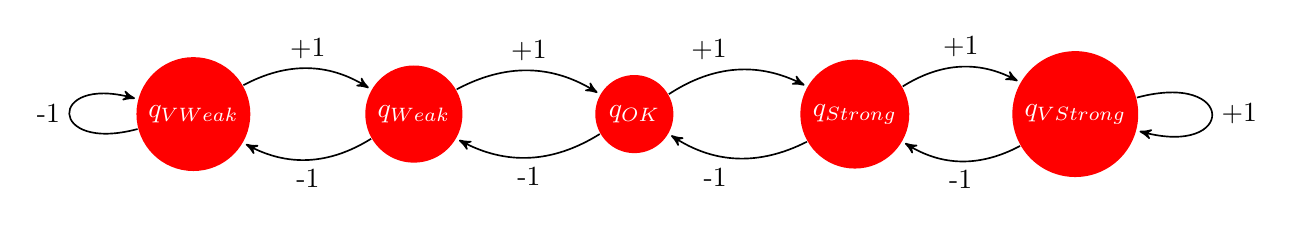
\begin{tikzpicture}[->,>=stealth',shorten >=1pt,auto,node distance=2.8cm,
                    semithick]
  \tikzstyle{every state}=[fill=red,draw=none,text=white]

  \node[state]         (A)                    {$q_{VWeak}$};
  \node[state]         (B) [right of=A]       {$q_{Weak}$};
  \node[state]         (C) [right of=B]       {$q_{OK}$};
  \node[state]         (D) [right of=C]       {$q_{Strong}$};
  \node[state]         (E) [right of=D]       {$q_{VStrong}$};

  \path (A) edge [bend left]  node {+1} (B)
                 edge [loop left]   node {-1}  (A) 
           (B) edge [bend left]  node {-1}  (A)
                 edge [bend left]  node {+1} (C)
           (C) edge [bend left]  node {-1}  (B)
                 edge [bend left]  node {+1} (D)
           (D) edge [bend left]  node {-1}  (C)
                 edge [bend left]  node {+1} (E)
           (E) edge [loop right] node {+1} (E)
                 edge [bend left]  node {-1}  (D);
\end{tikzpicture}




%% ==============================
\section{Evolution{\"a}rer Algorithmus}
%% ==============================

In diesem Abschnitt werden die Komponenten meines Algorithmus beschrieben, \dots

Im folgenden Abschnitt werden die folgenden Komponenten beschrieben, die f{\"u}r einen Evolution{\"a}ren Algorithmus verwendet werden. Dabei wurden die grundlegenden Bestandteile eines Evolution{\"a}ren Algorithmus beachtet und umgesetzt. 

\paragraph*{Signal}
Der wichtigste Bestandteil des Algorithmus ist das Individuum, dass in diesem Fall ein Signal ist. Ein Signal bildet eine Vibration ab. 
Das bedeutet es besitzt Attribute, die die L{\"a}nge der Vibration und die St{\"a}rke einer Vibration repr{\"a}sentieren.

